%% Type de document et encodage de la police
\documentclass[a4paper]{article}
\usepackage[utf8x]{inputenc}
\usepackage[T1]{fontenc}
\usepackage[colorlinks=true, allcolors=black]{hyperref}
% \usepackage[french]{babel}

%% Initialise la taille des pages et des marges
\usepackage[a4paper, top=3cm, bottom=3cm, left=2cm, right=2cm, marginparwidth=2cm]{geometry}

%% Packs utiles
\usepackage{amsmath}
\usepackage{graphicx}

%% Commandes perso
\renewcommand{\arraystretch}{1.2} %% row 20% longer
\renewcommand{\contentsname}{Table des matières}

%% Pour les exemples
\usepackage{mdframed}
\newmdenv[topline=false, bottomline=false, rightline=false, skipabove=\topsep, skipbelow=\topsep]{example}

%% Pour les diagrammes
\usepackage{tikz}
\tikzstyle{incolore} = [rectangle, rounded corners, draw=black, minimum height=1cm, minimum width=3cm, text width=3cm, text centered]


\title{Sécurité Défensive}
\author{Grégoire Roumache}
\date{Octobre 2021}

\begin{document}

\maketitle \tableofcontents















\section{Initialiser le switch cisco}





\begin{enumerate}

\item Aller chercher la VM Windows Server 2019 sur le NAS, sur lequel on doit installer le rôle "Network Policy and Access Services" (pas obligé de le faire tout de suite - section 4.1 de l'énoncé). Il faut bien prendre cette VM parce qu'il y a déjà l'AD installé je suppose. Ce qu'on va faire, c'est utiliser un wizard pour y configurer un serveur Radius pour des connections 802.1X. \\
(\url{https://docs.microsoft.com/en-us/windows-server/networking/technologies/nps/nps-top}) \\
\textbf{Remarque}: désactiver le parefeu peut nous éviter des problèmes plus tard.

\begin{center} 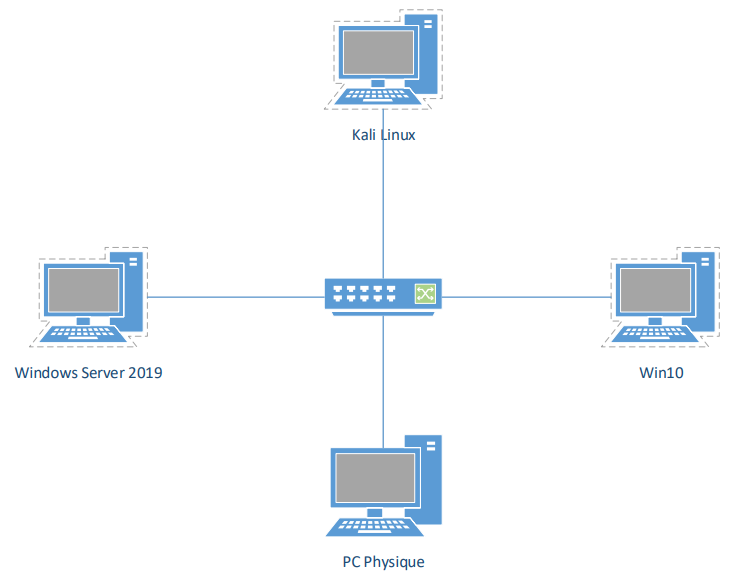
\includegraphics[width=0.75\linewidth]{images/topologie-01.PNG} \end{center}

\item Allumer le switch, se connecter au port console du switch avec un \textcolor{blue}{\textbf{bleu}} (le port est potentiellement à l'arrière du switch). Sur l'ordinateur, utiliser putty et le port COM1 ou COM2.

\item Effacer les configurations du switch:
\begin{enumerate}
    \item \texttt{enable}
    \item \texttt{delete flash:vlan.dat}
    \item \texttt{erase startup-config}
    \item \texttt{reload}
\end{enumerate}

\item Configuration de base du switch:
\begin{enumerate}
    \item \texttt{enable}
    \item \texttt{configure terminal}
    \item \texttt{line console 0}
    \item \texttt{logging synchronous}
    \item \texttt{exit}
    \item \texttt{write}
\end{enumerate}

\end{enumerate}















\section{Sécurisation de la couche 2 - port security}










\subsection{Synthèses/notes des années précédentes}





\begin{itemize}
    \item Méthode de débogage: \\ \url{https://github.com/groumache/latex-notes/tree/main/m%C3%A9thode-configuration-packet-tracer}
    \item Câblage au labo: \\ \url{https://github.com/groumache/latex-notes/tree/main/introduction-aux-r%C3%A9seaux-labo-Q2}
\end{itemize}











\subsection{Exploration des fonctionnalités du port-security}





\begin{enumerate}

\item Connecter le PC physique au switch avec un câble \textcolor{green}{\textbf{vert}}.

\item Mettre cette interface en mode access et shutdown toutes les autres interfaces (objectif = empêcher les trunks).
\begin{enumerate}
    \item \texttt{interface range f0/1-24}
    \item \texttt{switchport mode access}
    \item \texttt{switchport nonegotiate}
    \item \texttt{interface range f0/2-24} (ici, il faut mettre le bon range !)
    \item \texttt{shutdown}
\end{enumerate}

\item Activer le mode \textit{debug port-security} pour avoir plus d'infos: \texttt{debug port-security}.

\item Activer le switchport \textit{port-security} avec ses options par défaut sur cette interface.
\begin{enumerate}
    \item \texttt{interface <interface>} (interface = f0/1)
    \item \texttt{switchport port-security}
\end{enumerate}

\item Observer les informations affichées avec les commandes suivantes:
\begin{enumerate}
    \item \texttt{show port-security address}
    \item \texttt{show port-security interface <interface>}
\end{enumerate}
Sur base de ces informations, que risque-t-il d’arriver si vous connectez une machine virtuelle en pont sur cette même interface ? Faites le test.
\begin{example}
    Le \textit{violation mode} est \textit{shutdown}, ça signifie que si on connecte une machine virtuelle en pont sur ce même port, l'interface va s'éteindre.
\end{example}
Pour rétablir une interface verrouillée, vous devez commencer par corriger le problème pour ensuite, couper et rétablir l’interface (shutdown => no shutdown sur l’interface).

\end{enumerate}










\subsection{exercice 3.1 - port-security}





\begin{enumerate}

\item Configurer l’interface du switch pour qu’il permette au maximum à 4 adresses MAC de communiquer sur une interface. Ces adresses MAC doivent être sauvegardées dans la running-configuration du switch.
\begin{enumerate}
    \item \texttt{interface <interface>}
    \item \texttt{switchport port-security maximum <nb>}
    \item \texttt{switchport port-security mac-address [sticky]}
\end{enumerate}

\item  Lorsqu’une infraction est repérée sur une interface, le switch peut réagir de 3 façons différentes (switchport port-security violation \texttt{\{protect | restrict | shutdown\}}. Recherchez la différence entre ces 3 modes.
\begin{center}
    \begin{tabular}{|c|c|c|c|c|} \hline
        & \textbf{bloque le trafic} & \textbf{message syslog} & \textbf{++ compteur de violation} & \textbf{port shutdown} \\ \hline
        \textbf{protect}  & \textcolor{blue}{\textbf{oui}} & \textcolor{red}{\textbf{non}} & \textcolor{red}{\textbf{non}} & \textcolor{red}{\textbf{non}} \\
        \textbf{restrict} & \textcolor{blue}{\textbf{oui}} & \textcolor{blue}{\textbf{oui}} & \textcolor{blue}{\textbf{oui}} & \textcolor{red}{\textbf{non}} \\
        \textbf{shutdown} & \textcolor{blue}{\textbf{oui}} & \textcolor{blue}{\textbf{oui}} & \textcolor{blue}{\textbf{oui}} & \textcolor{blue}{\textbf{oui}} \\ \hline
    \end{tabular}
\end{center}
Commande: \texttt{switchport port-security violation \{protect | restrict | shutdown\}}.

\item Pour plus de sécurité, vous pourriez également entrer manuellement les seules adresses MAC autorisées à communiquer sur chaque interface.
\begin{itemize}
    \item statique: \texttt{switchport port-security mac-address <mac\_address>}
    \item dynamique + statique: \texttt{switchport port-security mac-address sticky <mac\_address>}
\end{itemize}

\item Dans un milieu où les utilisateurs changent d’interface de connexion régulièrement, vous pourriez utiliser les options présentes dans: \texttt{switchport port-security aging} pour gérer ces utilisateurs.
\begin{example}
    \begin{itemize}
        \item \texttt{[static]}: enable aging for configured secure address
        \item \texttt{[time <1-1440>]}: port security aging time in minutes
        \item \texttt{[type \{absolute|inactivity\}]}: port security aging type (default = absolute, inactivity = based on inactivity time period)
    \end{itemize}
\end{example}

\item Selon vous, quel type d’attaque êtes-vous capable de contrer grâce à cette protection ?
\begin{example}
    DHCP starvation.
\end{example}

\item Vérification: \texttt{show port-security}. Ensuite, enregistrer la configuration avec: \texttt{write} (ou: \texttt{do write}).

\end{enumerate}










\subsection{DHCP starvation}





\begin{enumerate}

\item Connecter la kali au switch (câble \textcolor{green}{\textbf{vert}}) et vérifier qu'elle est connecté \textbf{uniquement} au switch (en regardant les interfaces et en essayant de ping je suppose).

\item Revérifier que la kali n'est connectée qu'au switch (le prof insiste, peut-être lui demander quoi ?).

\item Configurer un serveur DHCP sur la machine Windows Server.
\begin{example}
    \begin{itemize}
        \item ip \textbf{statique} du serveur = 192.168.1.1
        \item range d'ip du dhcp = 192.168.1.(10-220)/24
    \end{itemize}
\end{example}

\item Retirer le switchport port-security de l’interface connectée à la machine virtuelle Kali:
\begin{enumerate}
    \item \texttt{interface <interface>}
    \item \texttt{no shutdown}
    \item \texttt{no switchport port-security}
\end{enumerate}

\item Avec Kali, lancez une attaque de type DHCP starvation avec le package Yersinia:
\begin{example}
    \texttt{sudo yersinia -G dhcp}
\end{example}

\item Observez la distribution des IP sur votre serveur; le pool est épuisé. Essayez d’obtenir une offre DHCP avec un autre client, cela devrait échouer. Après avoir observé ces résultats, refaites la manipulation en activant les options de sécurité adéquates sur le switch pour vous protéger de cette attaque (= activer le port-security, limiter le nombre de mac address, \textit{potentiellement} changer le mode de violation à quelque chose de plus restrictif). Ce type d’attaque est souvent suivi d’une deuxième partie, qui est l’introduction d’un Rogue DHCP 
server (comme expliqué en cours théorique btw).

\end{enumerate}










\subsection{protection des interfaces autorisant le DHCP}





\begin{enumerate}

\item À l’aide de la commande: \texttt{ip dhcp snooping}, préciser quels sont les interfaces sur lesquelles des serveurs DHCP se trouvent, vous protégeant ainsi des rogue DHCP.
\begin{enumerate}
    \item \texttt{interface <interface>}
    \item \texttt{ip dhcp snooping trust}
    \item vérification: \texttt{do show ip dhcp snooping | begin pps}
\end{enumerate}
\begin{example}
    Le DHCP snooping est une fonction de sécurité qui agit comme un pare-feu entre les hôtes non-approuvés et le serveur DHCP approuvé.
    Fonctionnalités:
    \begin{itemize}
        \item Filtre les messages non-valides.
        \item Limite le débit du trafic DHCP provenant de sources fiables et non-fiables.
        \item Gère une base de données DHCP contenant des informations sur les hôtes non-fiables avec des adresses IP louées.
        \item Utilise cette base de données pour valider les requêtes des hôtes non-fiables.
    \end{itemize}
    \textbf{Remarque}: les interfaces sont non-fiables par défaut.
\end{example}

\item Essayez à présent d’empêcher un rogue DHCP (depuis votre Kali par exemple) d’offrir des bails DHCP aux clients connectés au switch. Utilisez une deuxième interface du switch pour vous faciliter la vie.
\begin{example}
    Si on n'a pas deux machines, on peut mettre le trust sur un autre port et vérifier que le serveur DHCP de la machine windows server n'arrive pas à donner une adresse IP à une VM en pont connecté au switch sur la même interface.
\end{example}

\end{enumerate}















\section{Sécurisation de la couche 2 - connexion via l'AD/802.1x}










\subsection{Connexion via l'AD - windows server}





\begin{enumerate}

\item Installer et configurer le service AD (Active Directory):
\begin{enumerate}
    \item ouvrir le \textit{server manager}
    \item en haut à droite, cliquer sur \textit{manage}, puis sur \textit{add roles and features}
    \item à gauche dans \textit{server roles}, sélectionner \textit{active directory domain services}
    \item cliquer sur \textit{add features} dans la popup, puis continuer jusqu'à l'installation
    \item quand un signe danger apparaît en haut à droite, cliquer dessus
    \item cliquer sur \textit{promote this server to a domain controller}
    \item sélectionner l'option \textit{add a new forest}, et ajouter le nom de domaine (ex: \textit{ciscogreg.local})
    \item ensuite, ajouter le mot de passe DSRM: \textit{Tigrou007}, et terminer la configuration
\end{enumerate}

\item Aller dans \textit{active directory users and computers} et ajouter:
\begin{itemize}
    \item un groupe \texttt{cisco\_admin} à l'AD
    \item ajouter un utilisateur \texttt{admin1} dedans
\end{itemize}

\item Installer le service NPS (Network Policy Server) et ajouter le switch en tant que client radius:
\begin{enumerate}
    \item clic droit sur \textit{RADIUS Clients and Servers/RADIUS Clients}, puis cliquer sur \textit{New}
    \item ajouter un "friendly name" comme \textit{SwitchCisco}, l'IP du switch et un secret partagé comme \textit{Tigrou007}
\end{enumerate}

\item Ajouter une politique de connexion au service NPS:
\begin{itemize}
    \item dans NPS, clic droit sur \textit{nps/policies/network policies} et cliquer sur \textit{new}
    \item dans \textit{policy name}, mettre \textit{CiscoSwitchManagement}, puis cliquer sur \textit{next}
    \item ajouter une condition telle que seul le groupe windows \texttt{CISCOGREG$\backslash$cisco\_admin} soit concerné par la règle, puis cliquer sur \textit{next}
    \item ajouter la méthode d'authentification non-chiffrée \textit{PAP, SPAP}
    \item une fois arrivé dans \textit{configure constraints}, aller dans le sous-menu \textit{NAS Port Type}
    \item sélectionner \textit{async (modem)} et \textit{virtual (vpn)}, puis cliquer sur \textit{next}
    \item supprimer l'attribut \textit{Framed-Protocol} de valeur \textit{PPP}
\end{itemize}
\begin{center} 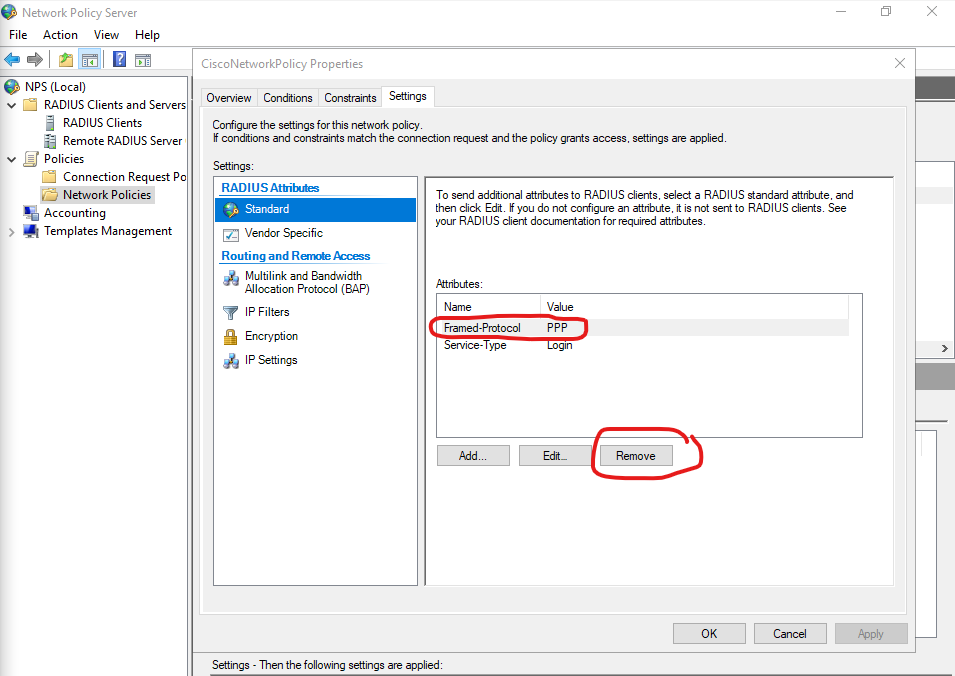
\includegraphics[width=0.90\linewidth]{images/remove-ppp.png} \end{center}

\item Configuration pour pouvoir se connecter en mode \texttt{enable}:
\begin{itemize}
    \item créer l'utilisateur \texttt{\$enab15\$} dans l'AD
    \item l'ajouter au groupe \texttt{cisco\_admin}
\end{itemize}
On fait ainsi parce que quand on essaie de passer en mode enable, le switch tente de se connecter avec cet utilisateur.
\begin{center} 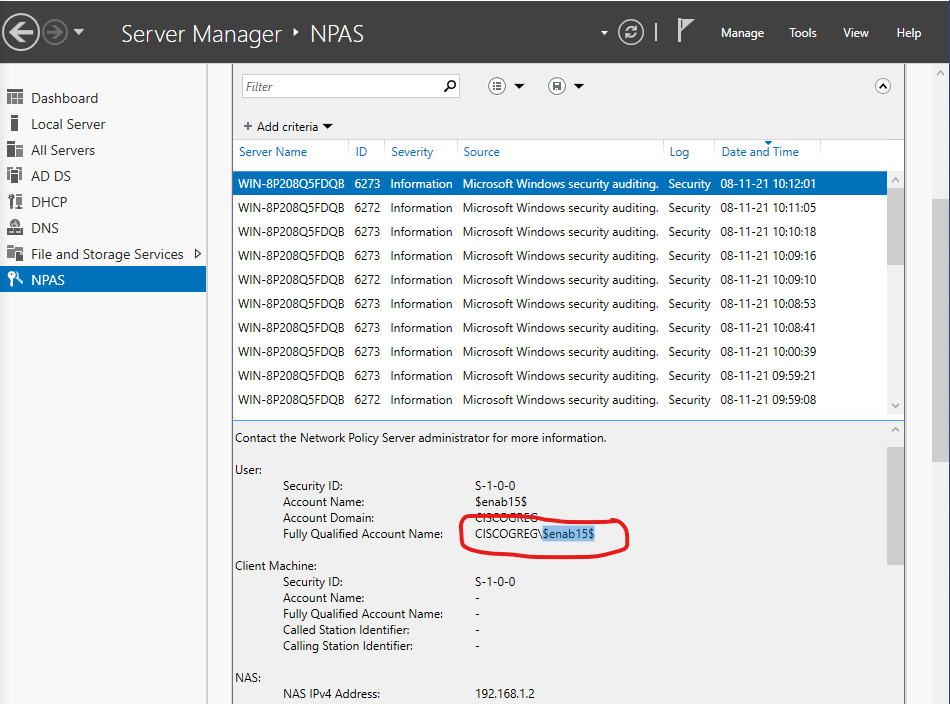
\includegraphics[width=0.85\linewidth]{images/logs-enab15.png} \end{center}

\item Si ce n'est toujours pas fait, désactiver le parefeu windows.

\end{enumerate}










\subsection{Connexion via l'AD - switch cisco}





\begin{enumerate}

\item Configurer l'interface VLAN1:
\begin{itemize}
    \item \texttt{interface vlan1}
    \item \texttt{no shutdown}
    \item \texttt{ip address 192.168.1.2 255.255.255.0}
\end{itemize}

\item Activer SSH:
\begin{itemize}
    \item \texttt{line vty 0 15}
    \item \texttt{transport input ssh}
    \item ajouter le domaine de l'AD: \texttt{ip domain-name <domain>} (\texttt{ip domain-name ciscogreg.local})
    \item ajouter un compte local pour se connecter au cas où: \texttt{username greg privilege 1 secret Tigrou007}
    \item \texttt{exit}
    \item \texttt{crypto key generate rsa}
\end{itemize}

\item Quelles sont les sous-commandes de \texttt{aaa} ?
\begin{enumerate}
    \item \texttt{aaa new-model}
    \item \texttt{aaa ?}
\end{enumerate}
\begin{center} 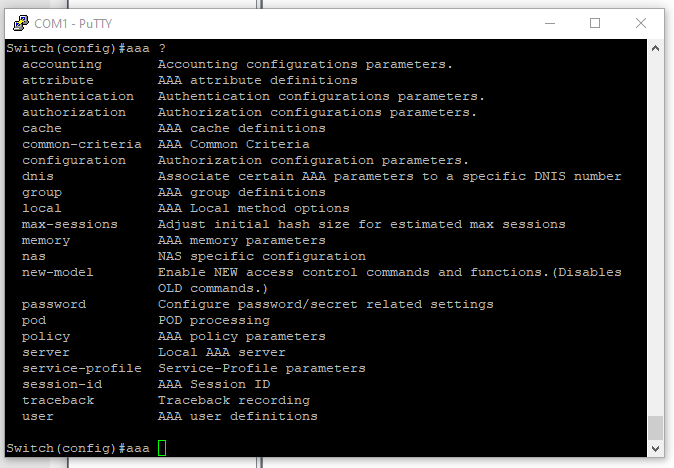
\includegraphics[width=0.80\linewidth]{images/aaa-options.png} \end{center}

\item Activer l'authentification avec le serveur radius:
\begin{enumerate}
    \item informations du serveur radius: \texttt{radius server host <server\_ip> key <shared\_secret>}
    \item autoriser l'authentification par mdp: \texttt{aaa authentication login default group radius enable}
    \item autoriser l'authentification par radius: \texttt{aaa authentication enable default group radius enable}
    \item donner les permissions enable aux utilisateurs connectés via radius: \texttt{aaa authorization exec default group radius if-authenticated}
\end{enumerate}

Essayez de vous connecter en SSH sur le switch. Utilisez le mot de passe de l'utilisateur \texttt{\$enab15\$} pour passer en mode enable.

\item En cas de problème, on peut consulter les logs du rôle Network Policy and Access Service (NPAS).
\begin{example}
    Pour vérifier, on peut faire \textit{exit} pour se déconnecter (pas besoin de débrancher/rebrancher le câble bleu) et se reconnecter. Si il y a des problèmes, on peut se connecter en SSH avec le compte local et reconfigurer.
\end{example}

\end{enumerate}

\begin{center} 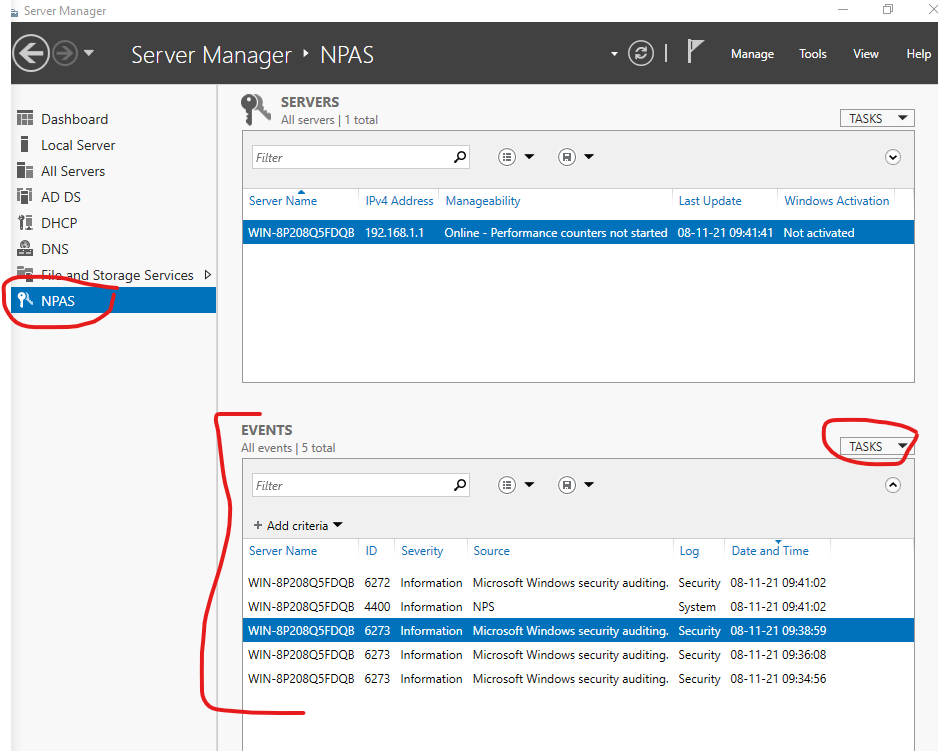
\includegraphics[width=0.90\linewidth]{images/logs-npas.png} \end{center}









\subsection{Authentification 802.1x - switch cisco}





\begin{enumerate}

\item Configurer l'authentification des machines se connectant à une des interfaces en dot1x:
\begin{enumerate}
    \item \texttt{dot1 system-auth-control}
    \item \texttt{aaa authorization network default group radius if-authenticated}
    \item \texttt{aaa authentication dot1x default group radius}
\end{enumerate}

\item Sur l'interface du switch où vous voulez configurer le 802.1x:
\begin{center} \begin{tabular}{|p{6.5cm}|p{7cm}|} \hline
    \begin{center} \textbf{vieux switch} \end{center} & \begin{center} \textbf{nouveau switch} \end{center} \\ \hline
    \begin{enumerate}
        \item \texttt{switchport mode access}
        \item \texttt{dot1x port-control auto}
        \item \texttt{debug dot1x all}
    \end{enumerate}
    &
    \begin{enumerate}
        \item \texttt{switchport mode access}
        \item \texttt{authentication port-control auto}
        \item \texttt{dot1x pae authenticator}
        \item \texttt{debug dot1x all}
    \end{enumerate} \\ \hline
\end{tabular} \end{center}

\end{enumerate}










\subsection{Authentification 802.1x - windows server}





\begin{enumerate}

\item Installer le rôle ADCS (Active Directory Certificate Service) sur la windows server. Il faut créer une CA (certificate authority) mais pas besoin de créer un certificat.

\item Se connecter au switch (avec le câble vert) avec un mot de passe:
\begin{enumerate}
    \item lancer: \texttt{services.msc}
    \item démarrer le service: \texttt{wired autoconfig}
    \item aller dans \texttt{ncpa.cpl} et suivre les captures d'écrans suivantes
\end{enumerate}

\end{enumerate}
\begin{center} 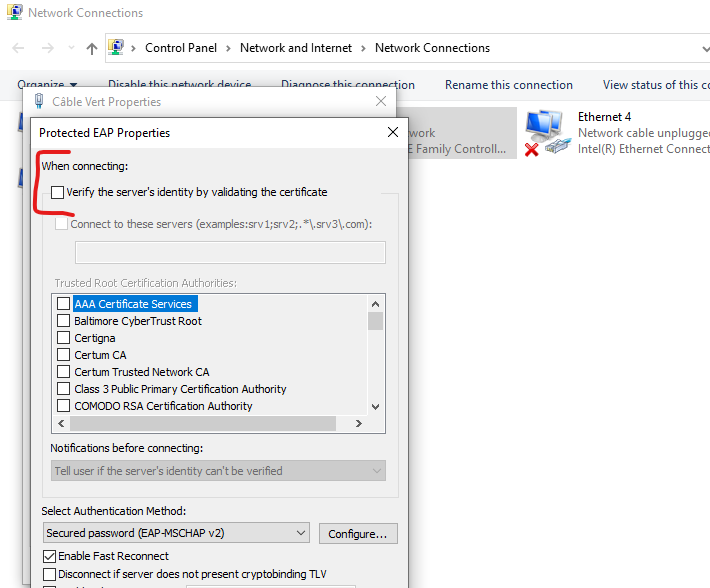
\includegraphics[width=0.75\linewidth]{images/connect-03.png} \end{center}
\begin{center} 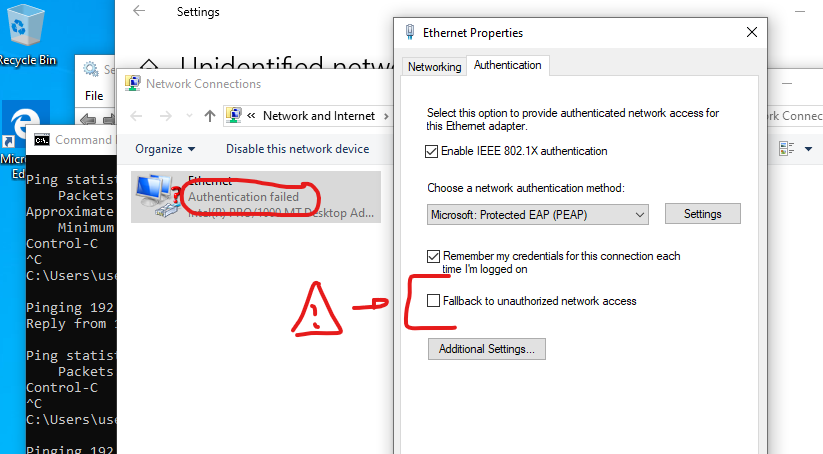
\includegraphics[width=0.90\linewidth]{images/connect-02.png} \end{center}
\begin{center} 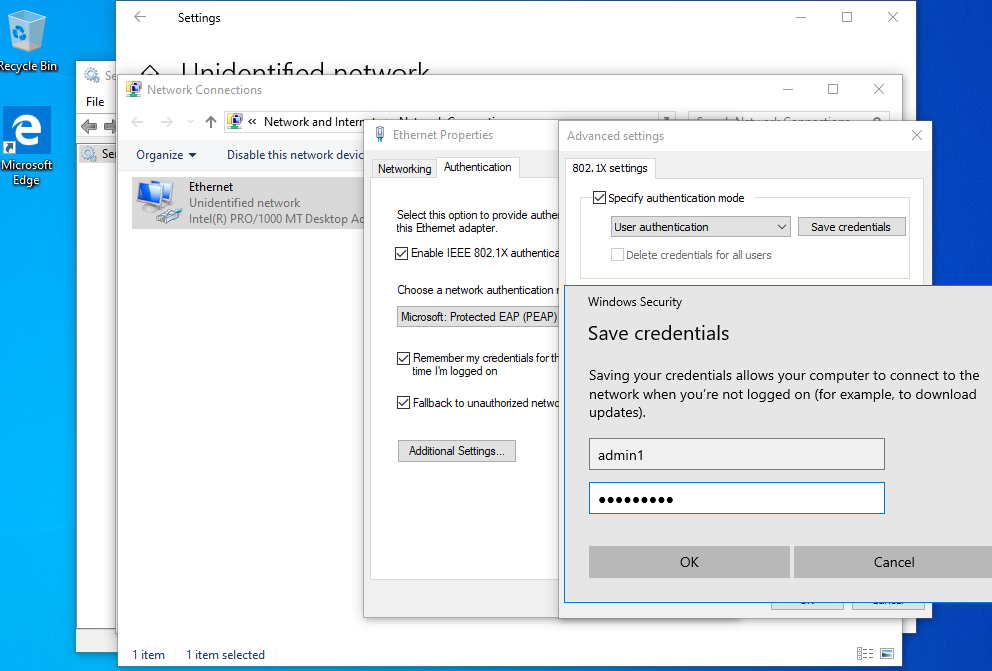
\includegraphics[width=0.90\linewidth]{images/connect-01.png} \end{center}










\subsection{Assignation automatique de VLAN}





Objectif = changer automatiquement le VLAN du port en fonction du groupe auquel l’utilisateur connecté appartient.

\begin{enumerate}

\item Sur le switch, créer les 3 vlans:
\begin{itemize}
    \item \texttt{vlan <number>}
    \item \texttt{name <name>}
\end{itemize}

\item Sur le serveur, aller dans l'\textit{active directory users and computers} et créer les 3 groupes (ex: \textit{vlan10}) et 3 utilisateurs (ex: \textit{user-vlan10}) pour chaque groupe.

\item Installer le service DHCP et créer 3 réseaux, 1 pour chaque vlan:
\begin{enumerate}
    \item dans la fenêtre de gestion du DHCP, faire un clic droit sur \textit{<server>.ciscogreg.local/ipv4}
    \item cliquer sur \textit{new scope}, dans \textit{name} entrer \textit{vlan10}
    \item entrer le range d'ip suivant: \textit{192.168.10.10} - \textit{192.168.10.250}
    \item pas besoin d'entrer une default gateway vu qu'on n'a pas de routeur
\end{enumerate}

\item Ouvrir \textit{Network Policy Server}
\begin{enumerate}
    \item aller dans \textit{Policies/Network Policies}
    \item créer une nouvelle policy \textit{CiscoVlan10}
    \item ajouter le groupe windows \textit{vlan10}
    \item ajouter la méthode d'authentification \textit{PAP, SPAP}
    \item dans \textit{nas port type}, ajouter \textit{async (modem)} et \textit{virtual (vpn)}
    \item retirer l'attribut \textit{Framed-Protocol} de valeur \textit{PPP}
    \item ajouter les attributs suivants (access type = 802.1x):
    \begin{center} \begin{tabular}{ll} \hline
        \textbf{Attribut}   & \textbf{Valeur} \\ \hline
        Tunnel-Type         & 802.1x - Virtual LANs (VLAN) \\
        Tunnel-Medium-Type  & 802.1x - 802 (includes all 802 media ...) \\
        Tunnel-Pvt-Group-ID & 10 (10 = numéro du vlan)\\ \hline
    \end{tabular} \end{center}
\end{enumerate}

\item Sur la windows client (qui se connecte avec le câble vert au switch), démarrer le service \textit{WLAN AutoConfig} dans \textit{services.msc}.

\end{enumerate}










\subsection{Authentification par certificat}





\textcolor{red}{\textbf{Pas à l'examen.}}















\newpage \section{Palo Alto - Bases}










\subsection{Topologie \& Explications sur le labo}





\begin{itemize}
    \item Topologie:
    \begin{center} 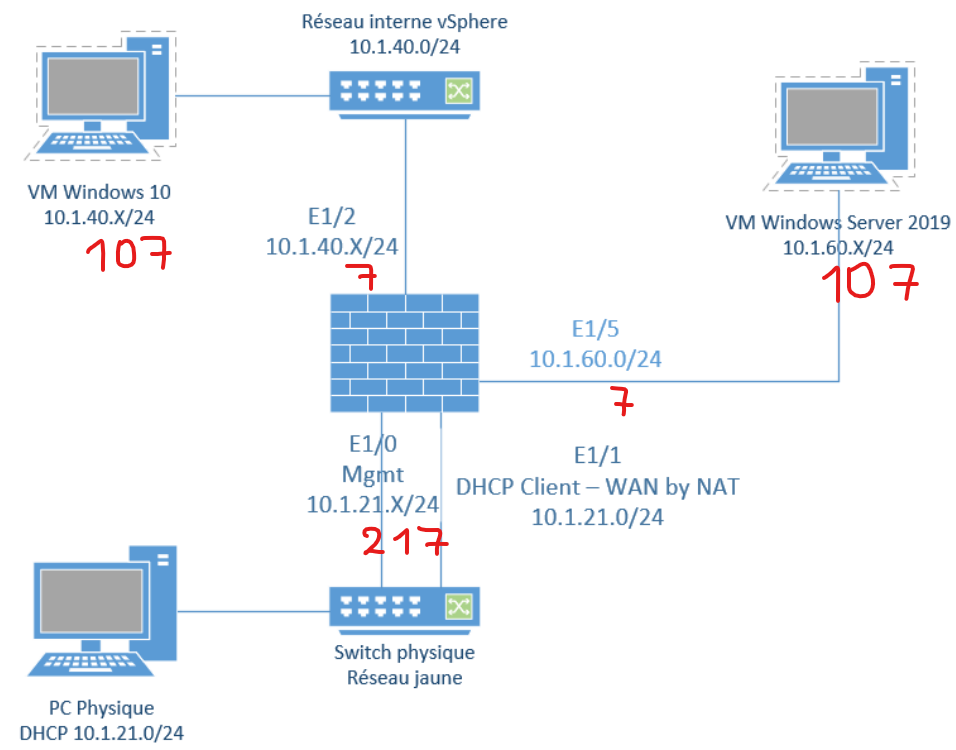
\includegraphics[width=0.75\linewidth]{images/topologie-02.png} \end{center}
    \item L'interface 0 (l'interface de management) est déjà configurée, on y accède via l'interface web, pas besoin de faire des changements.
    \item Une fois qu'on a configuré le parefeu pour que les machines puissent se ping et accéder à internet, il faudra suivre le chapitre User-ID de palo alto (l'user-id agent est sur moodle).
    \item L'objectif final est de pouvoir vérifier l'identité/les accès àpd utilisateurs de l'AD.
    \item Pour se connecter à vsphere, il faut utiliser ces identifiants: \texttt{Student@vsphere.local - Tigrou007=}, à l'adresse: \texttt{https://10.1.31.191/}.
    \item Pour se connecter à l'interface web de palo alto, il faut aller sur: \texttt{https://<ip>/} (dans mon cas: \texttt{https://10.1.21.217/}) et utiliser les identifiants: \texttt{admin - admin}.
    \item On peut ouvrir les machines windows, à partir de l'interface vsphere comme ceci:
    \begin{center} 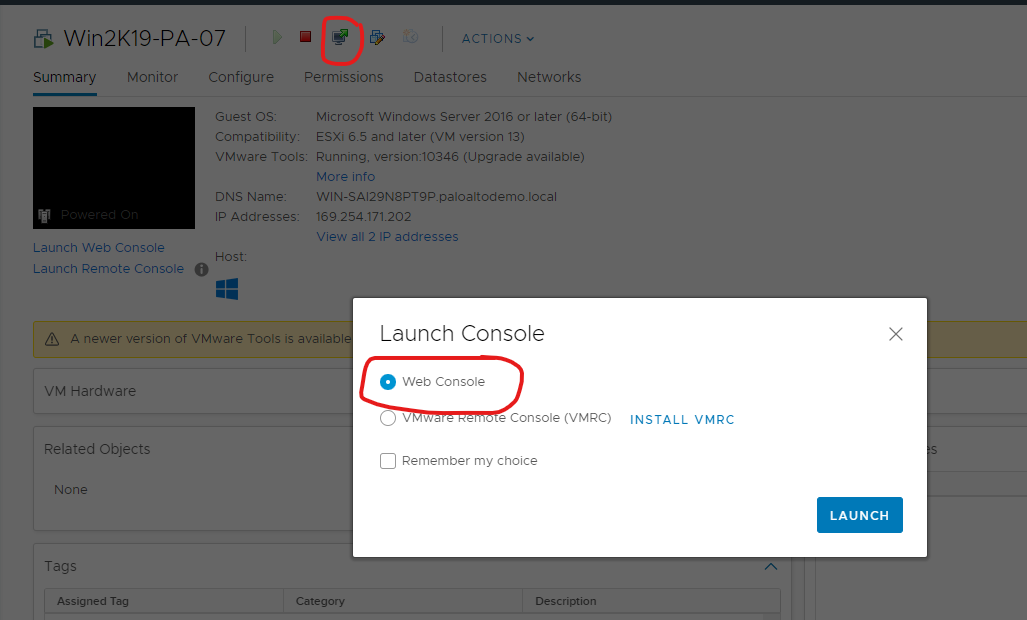
\includegraphics[width=0.80\linewidth]{images/web-console.png} \end{center}
    \item Enfin, il faut charger une configuration vide dans palo alto comme ceci:
\end{itemize}
\begin{center} 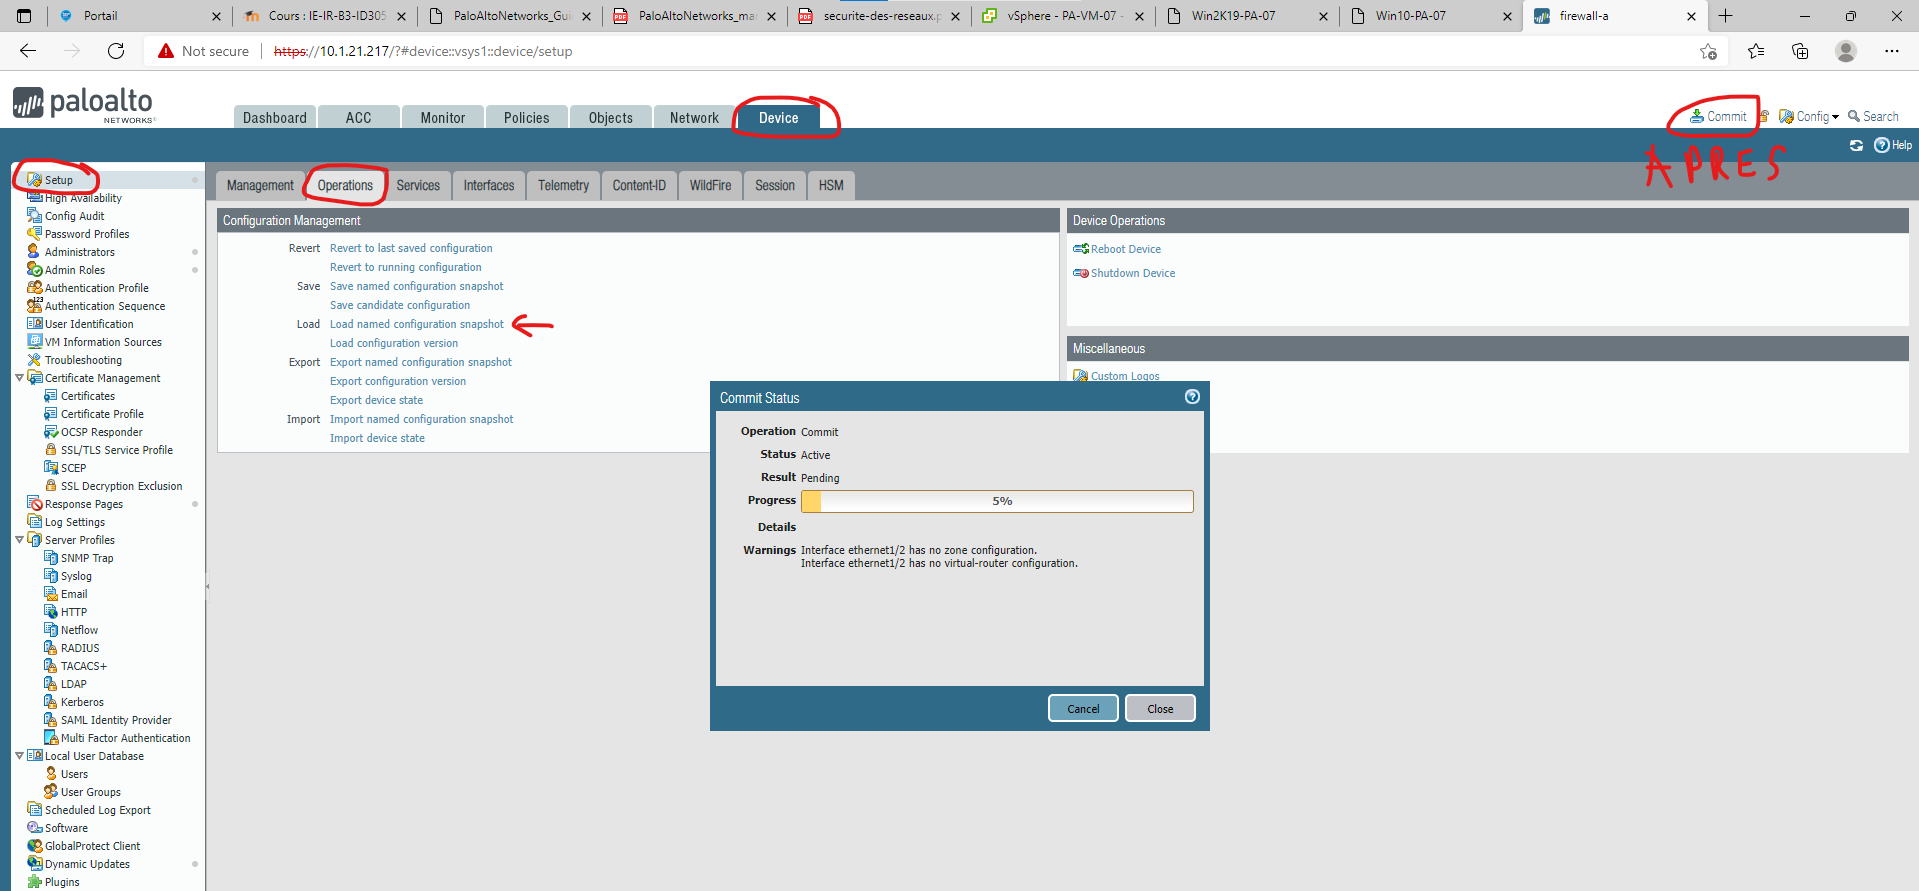
\includegraphics[width=0.99\linewidth]{images/load-config.png} \end{center}










\newpage \subsection{Configuration réseau de base}





\begin{enumerate}
    \item Créer les 4 zones (zone-client, zone-server, zone-management, zone-wan).
    \begin{example}
        Dans \texttt{network/zones}:
        \begin{itemize}
            \item name = zone-client
            \item type = layer 3
        \end{itemize}
    \end{example}
    \item Créer des \textit{interface management profile} (pour autoriser le ping et autre).
    \begin{example}
        Dans \texttt{network/network profiles/interface mgmt}:
        \begin{itemize}
            \item name = ping-and-response-pages
            \item network services = ping, response pages
        \end{itemize}
    \end{example}
    \item Créer un routeur virtuel pour router le trafic entre les interfaces.
    \begin{example}
        Dans \texttt{network/virtual routers}:
        \begin{itemize}
            \item name = routeur-virtuel
            \item interfaces = ethernet1/1, ethernet1/2, ethernet1/5
        \end{itemize}
    \end{example}
    \item Configurer les interfaces ethernet.
    \begin{example}
        Dans \texttt{network/interfaces/ethernet}:
        \begin{itemize}
            \item interface name = ethernet1/1
            \item comment = server-side
            \item interface type = layer 3
            \item virtual router = routeur-virtuel
            \item security zone = server-side
            \item ipv4/ip = 10.1.60.7/24 (ne pas mettre d'ip pour les interfaces en dhcp)
            \item advanced/management profile = ping-and-response-pages
        \end{itemize}
    \end{example}
    \item Créer 2 politiques de source nat (1 pour la zone client et 1 pour la zone serveurs).
    \begin{example}
        Dans \texttt{policies/nat}:
        \begin{itemize}
            \item general/name = nat-client-zone
            \item original packet/source zone = client-zone
            \item original packet/destination zone = wan
            \item original packet/destination interface = ethernet1/1
            \item translated packet/translation type = dynamic ip and port
            \item translated packet/address type = interface address
            \item translated packet/interface = ethernet1/1
        \end{itemize}
    \end{example}
    \item Créer des politiques de sécurité pour:
    \begin{itemize}
        \item autoriser le trafic vers internet (vers le wan)
        \item autoriser le trafic entre les zones internes
    \end{itemize}
    \begin{example}
        Dans \texttt{policies/security}:
        \begin{itemize}
            \item general/name = client-server-to-wan
            \item source/zone = client-zone, server-zone
            \item destination/zone = wan
        \end{itemize}
    \end{example}
    \item Commit tous les changements et tester la connectivité avec internet et entre les machines.
\end{enumerate}















\subsection{Configuration pour ajouter une machine de la zone client dans l'AD dans la zone serveur}





\begin{enumerate}
    \item Modifier la politique de sécurité qui autorise le trafic entre les zones client et serveur.
    \begin{example}
        Dans l'onglet \texttt{application}:
        \begin{itemize}
            \item ntp
            \item dns
            \item ms-netlogon
            \item kerberos
            \item ldap
            \item msrpc
            \item active-directory
            \item netbios-ss
            \item ms-ds-smb-base
            \item ms-ds-smbv2
            \item ms-ds-smbv3
            \item net.tcp
            \item netbios-ns
            \item netbios-dg
        \end{itemize}
    \end{example}
    \item Sur la windows server contenant l'active directory, trouver le nom de domaine de l'AD.
    \item Modifier le DNS de la windows 10 (il faut que ce soit l'ip de la windows server).
    \item Ajouter la windows 10 à l'AD.
    \begin{example}
        Ouvrir le \textit{control panel} sur la windows 10,
        \begin{enumerate}
            \item aller dans \textit{system and security}, puis dans \textit{system}
            \item à droite, cliquer sur \textit{change settings}, puis sur le bouton \textit{change}
            \item sélectionner le bouton radio \textit{domain}
            \item entrer le nom du domaine (ici, \textit{paloaltodemo.local}), puis appuyer sur \textit{ok}
            \item se connecter avec un compte de l'AD (ici, \textit{Administrator - Tigrou007=})
        \end{enumerate}
    \end{example}
\end{enumerate}














\newpage \section{Palo Alto - UserID (Active Directory)}










\subsection{Configuration de la windows server}





\begin{enumerate}
    \item ouvrir \textit{active directory users and computers} et créer un compte dans le domaine sous \textit{managed service accounts} (ex: \textit{greg-user-id})
    \item toujours dans \textit{managed service accounts}, créer un groupe (ex: \textit{group-user-id}) et y ajouter l'utilisateur créé
    \item ouvrir \textit{local security policy} (avec: \texttt{gpedit.msc}) et aller dans \textit{local policies/user rights assignment/log on as a service} et ajouter l'utilisateur créé (ex: \textit{<domaine>$\backslash$greg-user-id})
    \item ouvrir \textit{group policy management} (avec: \texttt{gpmc.msc}) et modifier la \textit{default domain policy}
    \item dans la fenêtre \textit{group policy management editor}, modifier la règle \textit{computer configuration/policies/windows settings/security settings/local policies/user rights assignments/log on as a service} et ajouter l'utilisateur créé (ex: \textit{<domaine>$\backslash$greg-user-id})
    \item télécharger \textit{paloalto-useragent-install.msi} qui se trouve dans le nas
    \begin{example}
        \begin{itemize}
            \item \texttt{$\backslash\backslash$10.1.21.204$\backslash$TI-Student$\backslash$IR305}
            \item Student - Tigrou007
        \end{itemize}
    \end{example}
    \item installer l'agent user-id et aller dans \textit{C:$\backslash$Program Files (x86)$\backslash$Palo Alto Networks}
    \begin{example}
        \begin{itemize}
            \item faire un clic droit sur le dossier \textit{User-ID Agent} et aller dans \textit{propriétés}
            \item aller dans l'onglet \textit{security}, cliquer sur \textit{edit}
            \item mettre comme owner l'utilisateur créé (ex: \textit{<domaine>$\backslash$greg-user-id}) et lui donner toutes les permissions
        \end{itemize}
    \end{example}
    \item ouvrir \textit{user-id agent} et aller dans \textit{user identification/discovery}
    \begin{example}
        \begin{enumerate}
            \item ajouter un serveur:
            \begin{itemize}
                \item name = server-user-id
                \item server address = <ip-pao-alto>
                \item server type = microsoft active directory
            \end{itemize}
            \item ajouter 2 configurations réseau (1 pour le réseau client, 1 pour le réseau serveur):
            \begin{itemize}
                \item names = server-network-user-id, client-network-server-id
                \item network address = 10.1.60.0/24, 10.1.40.0/24
            \end{itemize}
        \end{enumerate}
    \end{example}
    \item aller dans \textit{user identification/setup}, cliquer sur \textit{edit}, aller dans l'onglet \textit{client probing}, décocher les cases
    \item désactiver le parefeu de la windows server
\end{enumerate}










\subsection{Configuration de la Palo Alto}





\begin{enumerate}
    \item Activer l'User Identification (= User-ID):
    \begin{example}
        Dans \texttt{network/zones}:
        \begin{itemize}
            \item éditer la zone client
            \item cocher la case \textit{enable user identification}
        \end{itemize}
    \end{example}
    \item Ajouter un profil serveur LDAP:
    \begin{example}
        Dans \texttt{device/server profiles/ldap}:
        \begin{itemize}
            \item profile name = ldap-server-profile
            \item server list/name = ldap-server
            \item server list/ldap server = <ip-windows-server>
            \item server list/port = 389
            \item type = active-directory
            \item base dn = DC=paloaltodemo,DC=local
            \item bind dn = CN=Administrator,CN=Users,DC=paloaltodemo,DC=local
            \item password = <mdp-admin-domaine>
            \item décocher la case \textit{require ssl/tls secured connection}
        \end{itemize}
    \end{example}
    \item Ajouter une configuration de group-mapping:
    \begin{example}
        Dans \texttt{device/user identification/group mapping settings}:
        \begin{itemize}
            \item name = group-mapping-user-id
            \item server profile = ldap-server-profile
            \item group include list = ajouter le groupe d'utilisateurs autorisé
        \end{itemize}
    \end{example}
    \item Ajouter une configuration de user-mapping (\texttt{device/user identification/user mapping}).
    \item Ajouter un user-id agent:
    \begin{example}
        Dans \texttt{device/user identification/user-id agents}:
        \begin{itemize}
            \item name = agent-user-id
            \item host = <ip-windows-server>
            \item port = 5007
            \item enabled = coché
        \end{itemize}
    \end{example}
    \item Modifier les configurations de routes de services:
    \begin{example}
        Dans \texttt{device/setup/services}, cliquer sur \texttt{service route configuration}:
        \begin{itemize}
            \item sélectionner \textit{customize}
            \item ldap, uid agent:
            \begin{itemize}
                \item source interface = <interface-windows-server>
                \item source address = <ip-sur-interface-windows-server>
            \end{itemize}
        \end{itemize}
    \end{example}
    \item Modifier la règle de sécurité d'accès à internet pour la restreindre aux utilisateurs de l'AD:
    \begin{example}
        Dans \texttt{policies/security}, modifier la règle d'accès à internet pour les clients:
        \begin{itemize}
            \item user/source user = paloaltodemo$\backslash$group-user-id
            \item user/source user = paloaltodemo$\backslash$greg-user-id
            \item user/source user = paloaltodemo$\backslash$Administrator
        \end{itemize}
    \end{example}
    \item Vérifier que tout fonctionne en se connectant en admin du domaine ou avec le compte service (\texttt{greg-user-id}) sur la windows 10 et essayer d'accéder à internet.
\end{enumerate}




















\end{document}
